\documentclass[xcolor=x11names,compress]{beamer}

%% General document %%%%%%%%%%%%%%%%%%%%%%%%%%%%%%%%%%
\usepackage{graphicx}
\usepackage{tikz}
\usepackage[utf8]{inputenc} 
\usepackage[francais]{babel}
\usetikzlibrary{decorations.fractals}
%%%%%%%%%%%%%%%%%%%%%%%%%%%%%%%%%%%%%%%%%%%%%%%%%%%%%%


%% Beamer Layout %%%%%%%%%%%%%%%%%%%%%%%%%%%%%%%%%%
\useoutertheme[subsection=false,shadow]{miniframes}
\useinnertheme{default}
\usefonttheme{serif}
\usepackage{palatino}

\setbeamerfont{title like}{shape=\scshape}
\setbeamerfont{frametitle}{shape=\scshape}

\setbeamercolor*{lower separation line head}{bg=DeepSkyBlue4} 
\setbeamercolor*{normal text}{fg=black,bg=white} 
\setbeamercolor*{alerted text}{fg=red} 
\setbeamercolor*{example text}{fg=black} 
\setbeamercolor*{structure}{fg=black} 
 
\setbeamercolor*{palette tertiary}{fg=black,bg=black!10} 
\setbeamercolor*{palette quaternary}{fg=black,bg=black!10} 

\renewcommand{\(}{\begin{columns}}
\renewcommand{\)}{\end{columns}}
\newcommand{\<}[1]{\begin{column}{#1}}
\renewcommand{\>}{\end{column}}
%%%%%%%%%%%%%%%%%%%%%%%%%%%%%%%%%%%%%%%%%%%%%%%%%%




\begin{document}


%%%%%%%%%%%%%%%%%%%%%%%%%%%%%%%%%%%%%%%%%%%%%%%%%%%%%%
%%%%%%%%%%%%%%%%%%%%%%%%%%%%%%%%%%%%%%%%%%%%%%%%%%%%%%
\section{\scshape Introduction}
\begin{frame}
\title{GNU Image Manipulation Program (GIMP)}
%\subtitle{SUBTITLE}
\author{
	PELLICER Marine ANDREU Paola\\
	{\it Licence 2 Informatique}\\
	
\includegraphics[height=4cm]{wilber}
}

\titlepage
\end{frame}

%%%%%%%%%%%%%%%%%%%%%%%%%%%%%%%%%%%%%%%%%%%%%%%%%%%%%%
%%%%%%%%%%%%%%%%%%%%%%%%%%%%%%%%%%%%%%%%%%%%%%%%%%%%%%
\begin{frame}{Gimp}
\tableofcontents
\end{frame}

\subsection{Qu'est-ce que c'est ? / Bibliothèques}
\begin{frame}{Qu'est-ce que c'est ? / Bibliothèques}
\begin{itemize}
\item Qu'est-ce que c'est?\\
~~~~~Outil d'édition et de retouches d'image
\end{itemize}
\begin{itemize}
\item Bibliothèques\\
~~~~~GTK(Gimp ToolKit)/GDK(Gimp Drawing Kit)\\
~~~~~GTK+
\end{itemize}
\end{frame}

%%%%%%%%%%%%%%%%%%%%%%%%%%%%%%%%%%%%%%%%%%%%%%%%%%%%%%
\subsection{Versions et améliorations}
\begin{frame}{Versions et améliorations}
\begin{itemize}
\item 0.54 : février 1996, version bêta
\end{itemize}
\begin{itemize}
\item 0.60 : juin 1996, version alpha, ajout des trousses GTK/GDK, calques, améliorations d'outils
\end{itemize}
\begin{itemize}
\item 0.99 : février 1997, nouvelle API rendant possible l'écriture de scripts, GTK+, mémoire virtuelle, XCF
\end{itemize}
\begin{itemize}
\item 1.0 : 5 juin 1998, version "finale" stable et mise sur le marché
\end{itemize}
\end{frame}

%%%%%%%%%%%%%%%%%%%%%%%%%%%%%%%%%%%%%%%%%%%%%%%%%%%%%%
\begin{frame}{Versions et améliorations}
\begin{itemize}
\item 1.2.0 : 25 décembre 2000, amélioration interface utilisateur
\end{itemize}
\begin{itemize}
\item 2.0 : interface utilisateur plus accessible, librairie GTK2+, Scripts en Python
\end{itemize}
\begin{itemize}
\item 2.2-2.6 : fonctions vectorielles de bases(GFig), modifications sur outils et interface
\end{itemize}
\begin{itemize}
\item 2.8+ : système multi-fenêtres
\end{itemize}
\end{frame}

%%%%%%%%%%%%%%%%%%%%%%%%%%%%%%%%%%%%%%%%%%%%%%%%%%%%%%
%%%%%%%%%%%%%%%%%%%%%%%%%%%%%%%%%%%%%%%%%%%%%%%%%%%%%%
\section{\scshape Images, formats et outils}
\subsection{Image}
\begin{frame}{Image}
\begin{itemize}
\item Image vectorielle : 
composée d'objets géométriques (segments, courbes) et auxquels on peut appliquer différentes transformations (rotations, mise à l'échelle).
\end{itemize}
\begin{itemize}
\item Image matricielle : juxtaposition de pixels de couleurs formant une image.
\end{itemize}
\end{frame}
%%%%%%%%%%%%%%%%%%%%%%%%%%%%%%%%%%%%%%%%%%%%%%%%%%%%%%
\begin{frame}{Image}
\begin{center}
	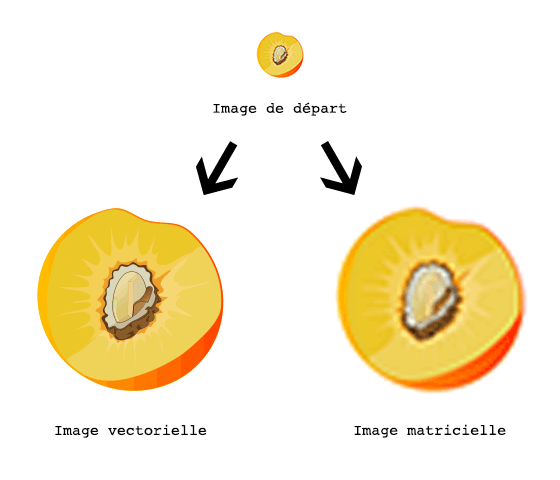
\includegraphics[height=7cm]{vecteur-vs-matricielle}
	\end{center}
\end{frame}
%%%%%%%%%%%%%%%%%%%%%%%%%%%%%%%%%%%%%%%%%%%%%%%%%%%%%%
\begin{frame}{Image}
\begin{itemize}
\item Résolution : sert à mesurer la qualité de l’image.\\
~~~~Plus il y a de pixels plus la qualité de l'image est grande.\\
~~~~La résolution est exprimée en pixels par pouces (ppp).
\end{itemize}
\begin{itemize}
\item Couleur : GIMP possède des modes de couleurs avec des formats de codage de couleur différents. 
\\
\begin{text}
RGB (16 millions couleurs), CMYK (impression), niveaux de gris, mode indexé (256 couleurs, utilisé pour les Gif)
\end{text}
\end{itemize}
\end{frame}
%%%%%%%%%%%%%%%%%%%%%%%%%%%%%%%%%%%%%%%%%%%%%%%%%%%%%%
\begin{frame}{Image}
\begin{itemize}
\item Format : 
\begin{itemize}
\item jpg utilisé pour les photos ne supporte pas de transparence ou d’animation.
\end{itemize}
\begin{itemize}
\item pgn supporte la transparence et utilisé pour les logos. 
\end{itemize}
\begin{itemize}
\item gif animation et réduis en couleurs (256) 
\end{itemize}
\begin{itemize}
\item xcf format GIMP conserve les outils utilisés.
\end{itemize}
\end{itemize}
\begin{itemize}
\item GIMP supporte également le format Open Raster.
\end{itemize}
\end{frame}
%%%%%%%%%%%%%%%%%%%%%%%%%%%%%%%%%%%%%%%%%%%%%%%%%%%%%%
%%%%%%%%%%%%%%%%%%%%%%%%%%%%%%%%%%%%%%%%%%%%%%%%%%%%%%
\subsection{Outils de base}
\begin{frame}{Outils de base}
\begin{itemize}
\item Gimp possède plusieurs outils de dessin, dont le pinceau, le crayon, la gomme et le pot de peinture.

\end{itemize}
\begin{itemize}
\item Brosses, dégradés et textures, (GIMP possède par défaut 48 brosses, mais il est possible d'en créer ou d'en télécharger de nouvelles) \\GIMP traite les dégradés, il les intègre également dans ses outils comme les brosses et l'outil de remplissage.
\end{itemize}

\end{frame}

%%%%%%%%%%%%%%%%%%%%%%%%%%%%%%%%%%%%%%%%%%%%%%%%%%%%%%
\begin{frame}{Outils de base}
\begin{itemize}
\item Calques : GIMP possède une gestion des calques, pouvant rendre des couches de l'image visibles, invisibles ou transparentes.

\end{itemize}
\begin{itemize}
\item Outils de transformation comme la rotation, la perspective et le redimensionnement.

\end{itemize}
\end{frame}

%%%%%%%%%%%%%%%%%%%%%%%%%%%%%%%%%%%%%%%%%%%%%%%%%%%%%%
\begin{frame}{Outils de base}

\begin{itemize}
\item GIMP possède des outils de sélection rectangulaire, elliptique et à main levée. 

\end{itemize}

\begin{itemize}
\item Utilisation des chemins pour faire des sélections ou des tracés personnalisés. Les chemins peuvent être aussi utilisés pour créer des sélections complexes.

\end{itemize}
\end{frame}

%%%%%%%%%%%%%%%%%%%%%%%%%%%%%%%%%%%%%%%%%%%%%%%%%%%%%%
%%%%%%%%%%%%%%%%%%%%%%%%%%%%%%%%%%%%%%%%%%%%%%%%%%%%%%
\subsection{Scripts-Fu}
\begin{frame}{Scripts-Fu}
\begin{itemize}
\item Les script-Fu autonomes : ne nécéssitent pas de canevas déjà existant, créent eux-mêmes ce dont ils ont besoin.
\end{itemize}
\begin{itemize}
\item Les script-Fu images : scripts appliqués à une image.
\end{itemize}
\end{frame}


%%%%%%%%%%%%%%%%%%%%%%%%%%%%%%%%%%%%%%%%%%%%%%%%%%%%%%
%%%%%%%%%%%%%%%%%%%%%%%%%%%%%%%%%%%%%%%%%%%%%%%%%%%%%%
\section{\scshape Démonstration de certains outils}
\subsection{Présentation de l’interface}
\begin{frame}{Présentation de l’interface}

	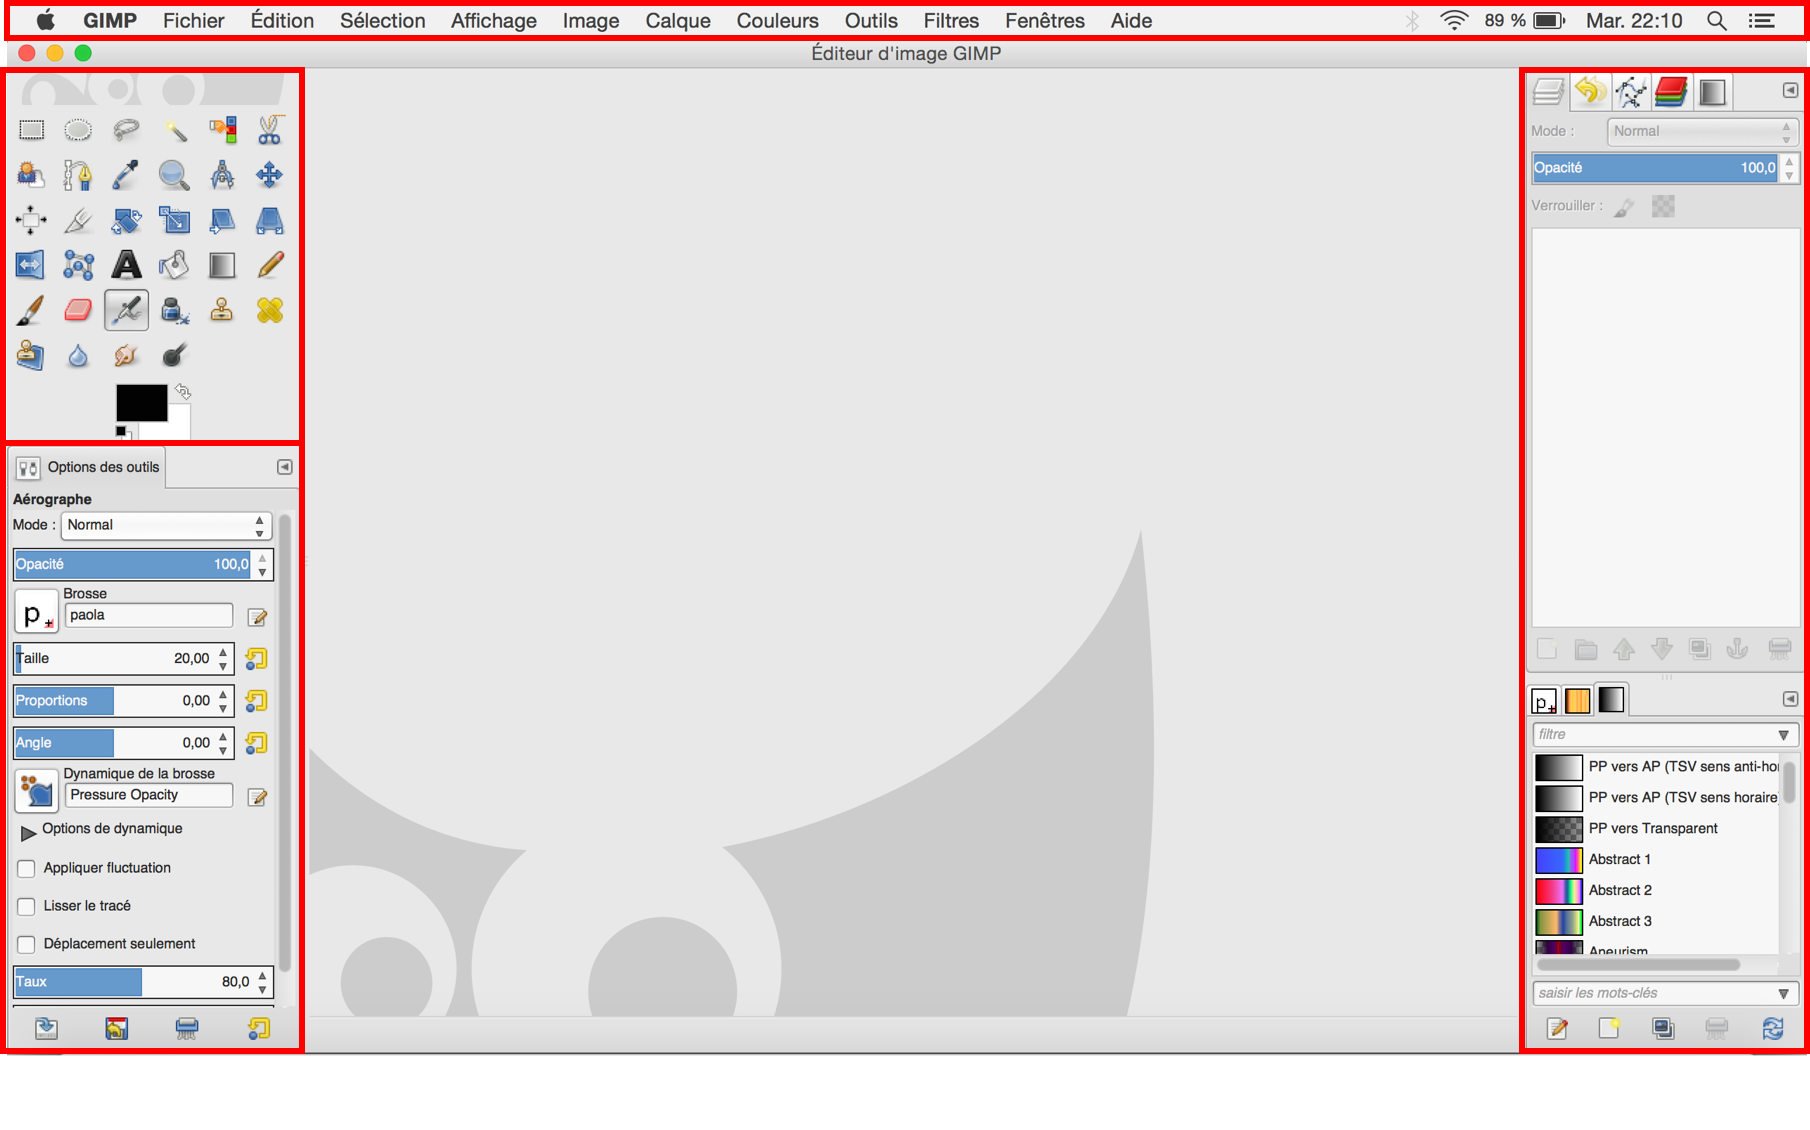
\includegraphics[height=7cm]{gimp}

\end{frame}


%%%%%%%%%%%%%%%%%%%%%%%%%%%%%%%%%%%%%%%%%%%%%%%%%%%%%%
%%%%%%%%%%%%%%%%%%%%%%%%%%%%%%%%%%%%%%%%%%%%%%%%%%%%%%
\subsection{Outils}
\begin{frame}{Outils}
\begin{itemize}
\item Sélection : Outil d'extraction du premier plan\\ 
\begin{itemize}
\item Délimiter grâce aux ancres l'objet à selectionner (laisser une marge autour de l'objet), choisir les couleurs que l'on souhaite conserver en déplaçant la souris sur la zone à garder, réajuster les couleurs avec la souris, cliquer sur l'image lorsque toutes les étapes sont finies.\\
\item Sélection$\ \to\ $inverser la sélection\\
\item Edition$\ \to\ $effacer\\
\end{itemize}
\begin{center}
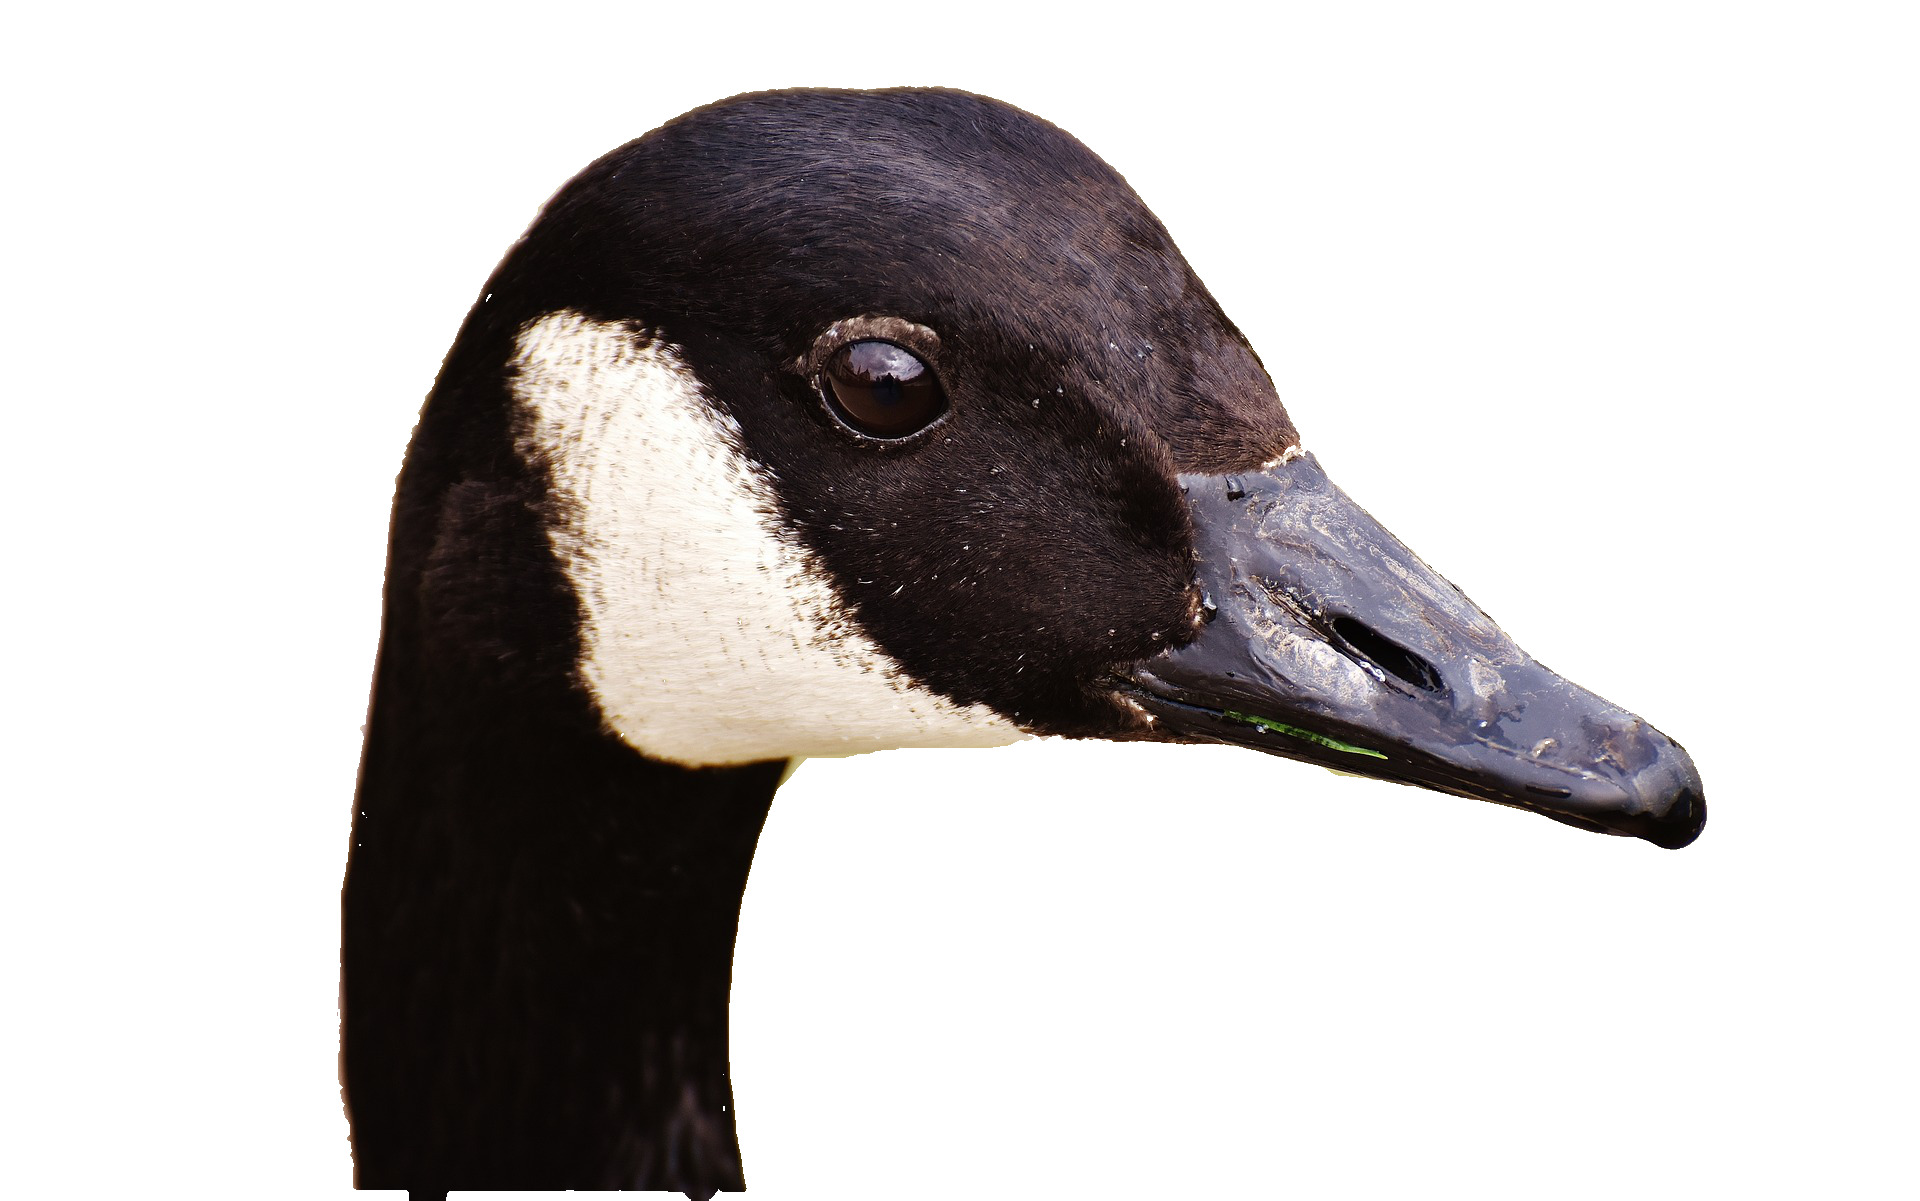
\includegraphics[height=3cm]{canard}
\end{center}
\end{itemize}
\end{frame}


%%%%%%%%%%%%%%%%%%%%%%%%%%%%%%%%%%%%%%%%%%%%%%%%%%%%%%
\begin{frame}{Outils}
\begin{itemize}
\item Calques \\
\begin{itemize}
\item Ouvrir l'image
\item Créer un calque et choisir la couleur d'arrière plan 
\item Le placer derrière l'image : Calque$\ \to\ $Pile$\ \to\ $descendre le calque
\item Créer un calque texte : dans la boite à outils
\item Fusionner les calques : image$\ \to\ $fusionner les calques visibles
\item Changer de mode de couleur : image$\ \to\ $mode$\ \to\ $niveaux de gris 
\end{itemize}
\begin{center}

\includegraphics[height=3.5cm]{ex1}
\end{center}
\end{itemize}
\end{frame}

%%%%%%%%%%%%%%%%%%%%%%%%%%%%%%%%%%%%%%%%%%%%%%%%%%%%%%
%%%%%%%%%%%%%%%%%%%%%%%%%%%%%%%%%%%%%%%%%%%%%%%%%%%%%%
\subsection{Scripts-Fu}
\begin{frame}{Scripts-Fu autonome}
\begin{itemize}
\item Code 
\begin{center}
	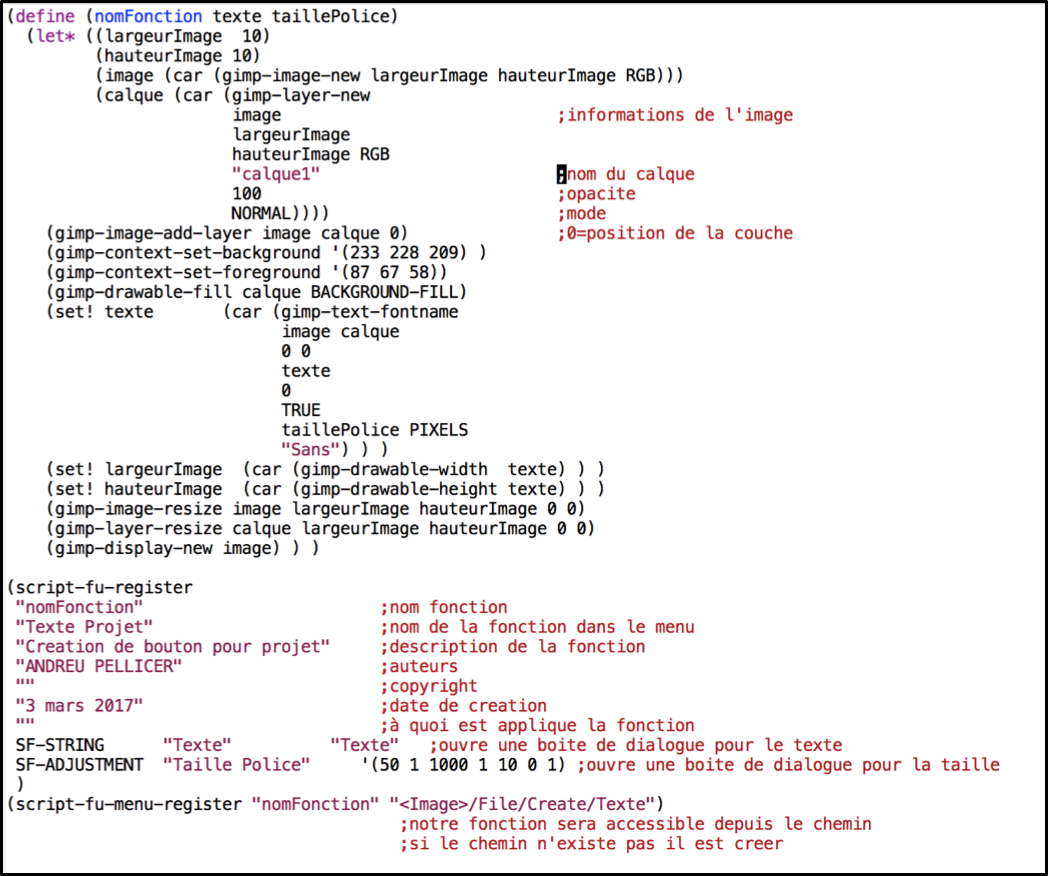
\includegraphics[height=5cm]{fonction}
	\end{center}
\end{itemize}
\begin{itemize}
\item Exemple \\

	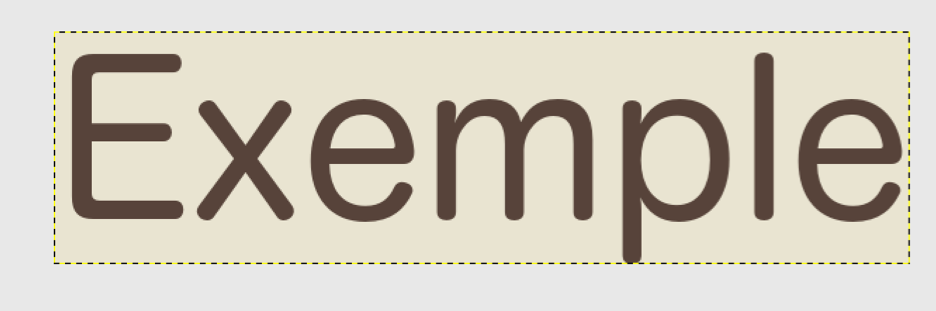
\includegraphics[height=1cm]{exemple}

\end{itemize}

\end{frame}

%%%%%%%%%%%%%%%%%%%%%%%%%%%%%%%%%%%%%%%%%%%%%%%%%%%%%%
%%%%%%%%%%%%%%%%%%%%%%%%%%%%%%%%%%%%%%%%%%%%%%%%%%%%%%
\section{\scshape Conclusion}
\subsection{Avantages et inconvénients}
\begin{frame}{Avantages et inconvénients}
\begin{itemize}
\item Gratuit et libre
\end{itemize}
\begin{itemize}
\item Manuel d'aide en français
\end{itemize}
\begin{itemize}
\item Facile d'utilisation et personnalisable
\end{itemize}
\end{frame}

\subsection{Oeuvres connues}
\usebackgroundtemplate{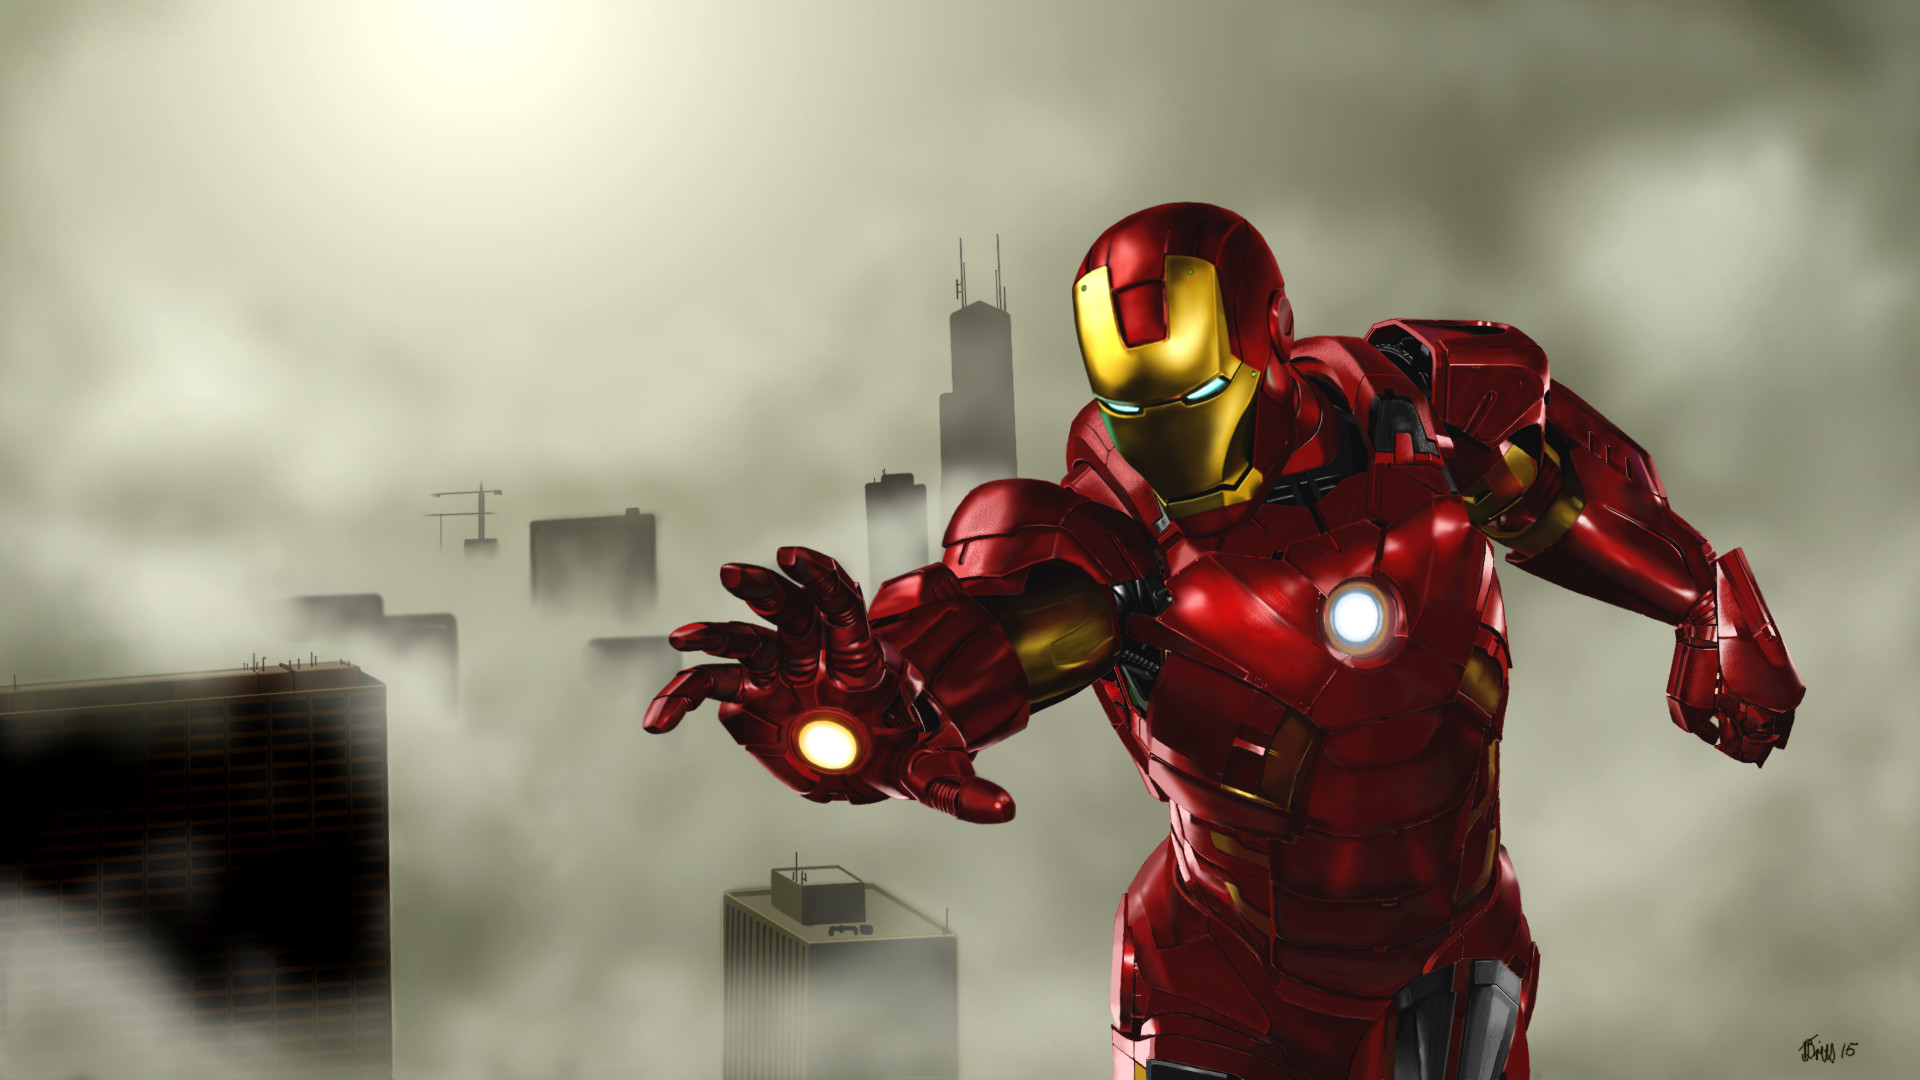
\includegraphics[width=\paperwidth, height = \paperheight]{iron-man}}
\begin{frame}
\end{frame}
\usebackgroundtemplate{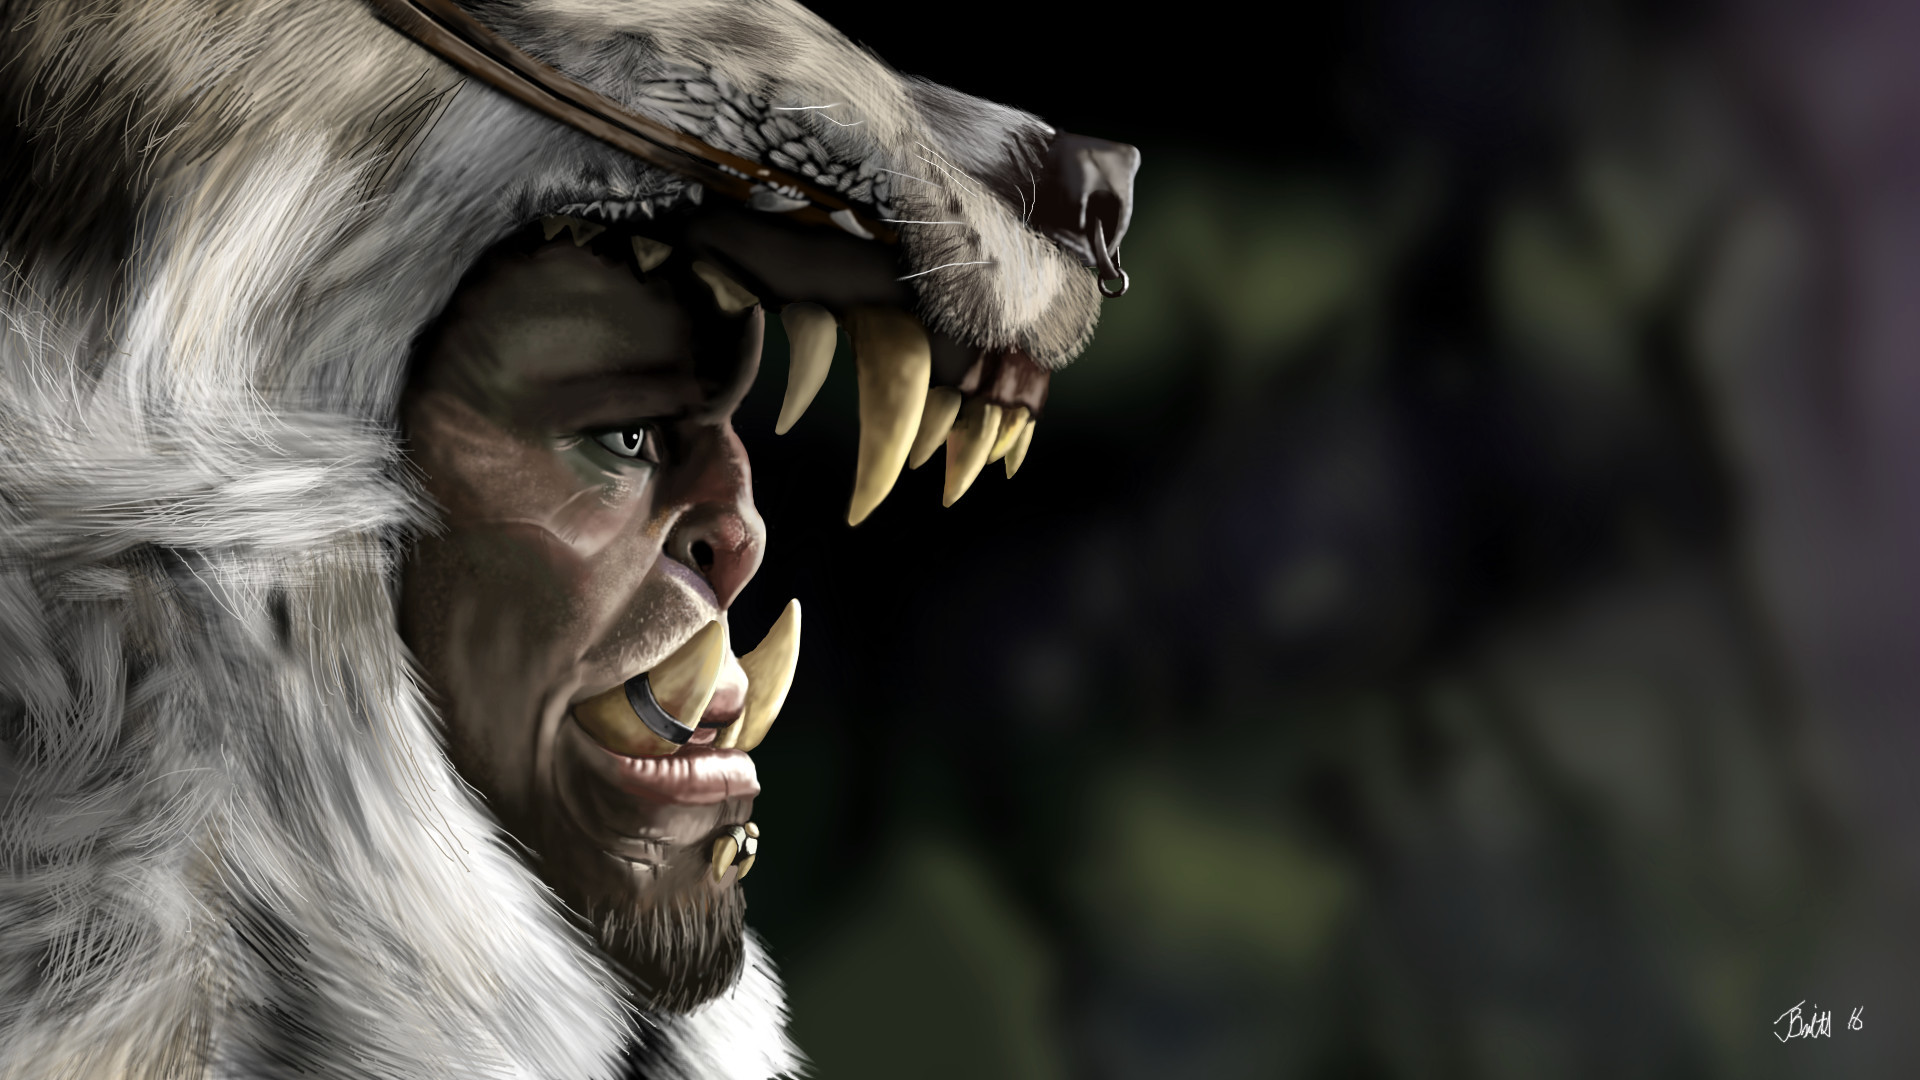
\includegraphics[width=\paperwidth, height = \paperheight]{durotan}}
\begin{frame}
\end{frame}
\end{document}